\documentclass{beamer}

\usepackage[utf8]{inputenc}
\usepackage{pdfpages}
\usepackage{listings}


\title{Determining a Cache Hit/Miss over RDMA}
\subtitle{A NetCAT Replication}
\author{Emerson Ford \and Calvin Lee}
\date{CS 6465 - Fall 2019}



\begin{document}
\frame{\titlepage}

\begin{frame}[t]
 \frametitle{NetCAT Overview}
 \begin{block}{Claim}
  Using RDMA over Infiniband, a remote host can measure if a remote memory access is served from LLC or from DRAM on a target host with DDIO enabled.
 \end{block}

 \begin{block}{Impact}
  Enables cache-timing based attacks (such as PRIME+PROBE) over the network which then enables attacks like SSH keystroke timing attacks.
 \end{block}

 \begin{block}{Key Replication Questions}
  \begin{enumerate}
   \item Is it actually possible to measure cache hit/cache hit on a remote memory access?
   \item If so, can we replicate their method of building a remote eviction set?
  \end{enumerate}
 \end{block}
\end{frame}

\begin{frame}
 \frametitle{Key Graph to Replicate}
 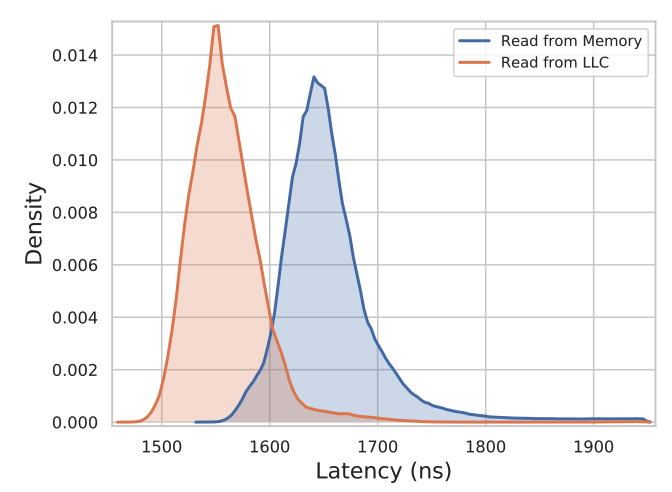
\includegraphics[width=\textwidth]{replication_graph.png}
\end{frame}

\begin{frame}
 \frametitle{RDMA Overview}

 \begin{enumerate}
  \item Server and client both register memory to be used for RDMA.
 \end{enumerate}

 \begin{block}{Reads}
  \begin{enumerate}
   \setcounter{enumi}{1}
   \item Client specifies a remote address and fires off `READ' verb.
   \item Client NIC communicates with remote NIC to read remote memory address (no CPU involvement).
   \item Client NIC places remote memory contents into client's registered memory.
  \end{enumerate}
 \end{block}

 \begin{block}{Writes}
  \begin{enumerate}
   \setcounter{enumi}{1}
   \item Client alters local registered memory.
   \item Client specifies a remote address and fires off `WRITE' verb.
   \item Client NIC communicates with remote NIC to write local memory contents at remote address (no CPU involvement).
  \end{enumerate}
 \end{block}

\end{frame}

\begin{frame}
 \frametitle{Other Key Facts}

 \begin{block}{DDIO}
  \begin{itemize}
   \item Reads can be served from LLC or DRAM. If served from DRAM, the memory is \textbf{not} loaded into LLC.
   \item Writes will load memory into the LLC if not already present.
   \item DDIO is ``restricted to 10\% of the last-level cache''.
  \end{itemize}
 \end{block}

 \begin{block}{Infiniband}
  \begin{itemize}
   \item DRAM access and LLC access for an Infiniband NIC should take longer than a CPU's access due to PCIe communication?
   \item Infiniband RDMA reads (on \texttt{apt080} and \texttt{apt083}) take 1900ns on average with 50ns standard deviation.
  \end{itemize}
 \end{block}
\end{frame}

\begin{frame}
 \frametitle{Timing Code}
 Read $\rightarrow$ Write $\rightarrow$ Read a remote address.



\end{frame}


\begin{frame}
 \frametitle{Problems}
 \begin{itemize}
  \item NUMA
  \item RDMA-enabled nodes are likely to be network-traffic intensive
  \item Prefetchers

 \end{itemize}
\end{frame}


\end{document}
